\documentclass[aspectratio=169,usenames,dvipsnames]{beamer}
\usetheme{metropolis}
%\usecolortheme[snowy,cautious]{owl}
\usecolortheme[snowy]{owl}
\metroset{block=fill}

% For regular math font
\usefonttheme[onlymath]{serif}

\usepackage{appendixnumberbeamer}
\usepackage{booktabs}
\usepackage{fancyvrb}
\usepackage{makecell}
\usepackage{xcolor}
%\usepackage{soul}
\usepackage[normalem]{ulem}
\usepackage{hyperref}
\hypersetup{colorlinks,allcolors=.,urlcolor=blue}
\usepackage{graphicx}
\usepackage{siunitx}
\usepackage[siunitx,europeanresistors,nooldvoltagedirection]{circuitikz}
\usepackage{amsmath}
\usepackage{amssymb}
\usepackage{color}
\usepackage{listings}

% For tikz
\colorlet{darkgreen}{OliveGreen}
\colorlet{darkred}{BrickRed}
% Not used
\definecolor{mygreen}{rgb}{0,0.6,0}
\definecolor{mygray}{rgb}{0.5,0.5,0.5}
\definecolor{mymauve}{rgb}{0.58,0,0.82}
\definecolor{myblue}{rgb}{0,0,1}
% For C
\definecolor{comment}{RGB}{0,128,0} % dark green
\definecolor{string}{RGB}{255,0,0}  % red
\definecolor{keyword}{RGB}{0,0,255} % blue

% Schematic elements colors
\tikzset{
  R/.append style={color=darkred, /tikz/text=black},
  battery1/.append style={color=darkred, /tikz/text=black},
  leDo/.append style={color=darkred, /tikz/text=black},
  short/.append style={color=darkgreen, /tikz/text=black},
  nos/.append style={color=darkred, /tikz/text=black},
  every vcc node/.style={color=darkred, /tikz/text=black},
  every ground node/.style={color=darkred, /tikz/text=black},
  %%% Pin element definition (crossed-out box)
  box/.style={
    rectangle, minimum size=0.5 cm, very thick, draw=black, color=darkred
  },
  pin/.style={
    box,
    append after command={
      [every edge/.append style={
        very thick,
        darkred,
        shorten >=\pgflinewidth,
        shorten <=\pgflinewidth,
      }]
      (\tikzlastnode.north west) edge (\tikzlastnode.south east)
      (\tikzlastnode.north east) edge (\tikzlastnode.south west)
    }
  }
}

% Fix dashs/hyphens in listings
\makeatletter
\lst@CCPutMacro\lst@ProcessOther {"2D}{\lst@ttfamily{-{}}{-{}}}
\@empty\z@\@empty
\makeatother

\newfontfamily\Bera{Bitstream Vera Sans Mono}[Scale=1]
\newfontfamily\TgCursor{TeX Gyre Cursor}[Scale=1]
\newfontfamily\Dejavu{DejaVu Sans Mono}[Scale=1]
%\newfontfamily\Consolas{Consolas}[Scale=0.85]
\newfontfamily\Consolas{Consolas}[Scale=1]

\lstdefinestyle{global} {
%  basicstyle=\fontfamily{cmvtt}\selectfont
%  basicstyle=\tiny\ttfamily,
%  basicstyle=\tiny\Dejavu,
  basicstyle=\tiny\Consolas,
  backgroundcolor=\color{white},
  commentstyle=\itshape\color{comment},
  stringstyle=\color{string},
  keywordstyle=\bfseries\color{keyword},
  %identifierstyle=\bfseries,
  numbers=left,
  numberstyle=\tiny,
  numbersep=5pt,
  frame=lines,
  breaklines=true,
  prebreak=\raisebox{0ex}[0ex][0ex]{\ensuremath{\hookleftarrow}},
  showstringspaces=false,
  upquote=true,
  tabsize=8,
  escapeinside=\`\`,
}

\lstdefinestyle{c} {
  escapeinside=\`\`,
}

\lstdefinestyle{make} {
  language=make,
  morekeywords={if,ifneq,else,elseif,endif},
}

\lstset {
  language=C,
  style=global,
}

% allowframebreaks numbering in the title
\newcounter{cont}
\makeatletter
\setbeamertemplate{frametitle continuation}{%
    \setcounter{cont}{\beamer@endpageofframe}%
    \addtocounter{cont}{1}%
    \addtocounter{cont}{-\beamer@startpageofframe}%
    (\insertcontinuationcount/\arabic{cont})%
}
\makeatother

\title{Kernel Course: Lecture 16}
\subtitle{Communicating with Hardware (part 1)}
\date{\today}
\author{Sam Protsenko}
\institute{GlobalLogic}

\begin{document}

\sisetup{
  math-rm = \mathrm,
  inter-unit-product = \ensuremath{{}\cdot{}},
  per-mode = fraction,
%  fraction-function = \tfrac,
%  unit-color = purple
}

\maketitle

\begin{frame}{Agenda}
  \setbeamertemplate{section in toc}[sections numbered]
  \tableofcontents[hideallsubsections]
\end{frame}

\section{Architecture Design}

\begin{frame}
  \frametitle{Objectives}
  \begin{itemize}
    \item Learn how to communicate with hardware \\
          (Hardware = SoC + Board + External)
    \item Grasp the whole development chain: \textbf{Hardware \textrightarrow{}
          Kernel \textrightarrow{} User space}
    \item Learn how to develop \textbf{upstreamable} and
          \textbf{production ready} driver
    \item Structure previously obtained knowledge:
    \begin{itemize}
      \item Get deeper understanding
      \item Learn missing parts
    \end{itemize}
    \item Prepare base for further development
  \end{itemize}
\end{frame}

\begin{frame}
  \frametitle{Design Requirements}
  \begin{itemize}

    \item Hardware:
    \begin{itemize}
      \item Prototyping on breadboard
      \item External LED and button
      \item Make it accessible via GPIOs
      \item Prepare HW info for development
    \end{itemize}

    \item Kernel:
    \begin{itemize}
      \item Device Tree (definition in dts; obtain in module)
      \item Control the LED and button (GPIO, interrupt)
      \item User-space interface (char dev, file ops)
      \item Power management
    \end{itemize}

    \item User space:
    \begin{itemize}
      \item Test driver via \texttt{echo} and \texttt{cat}
      \item Develop application for testing driver
    \end{itemize}
  \end{itemize}
\end{frame}

\begin{frame}
  \frametitle{Software Archictecture}
  \begin{figure}
    \centering
    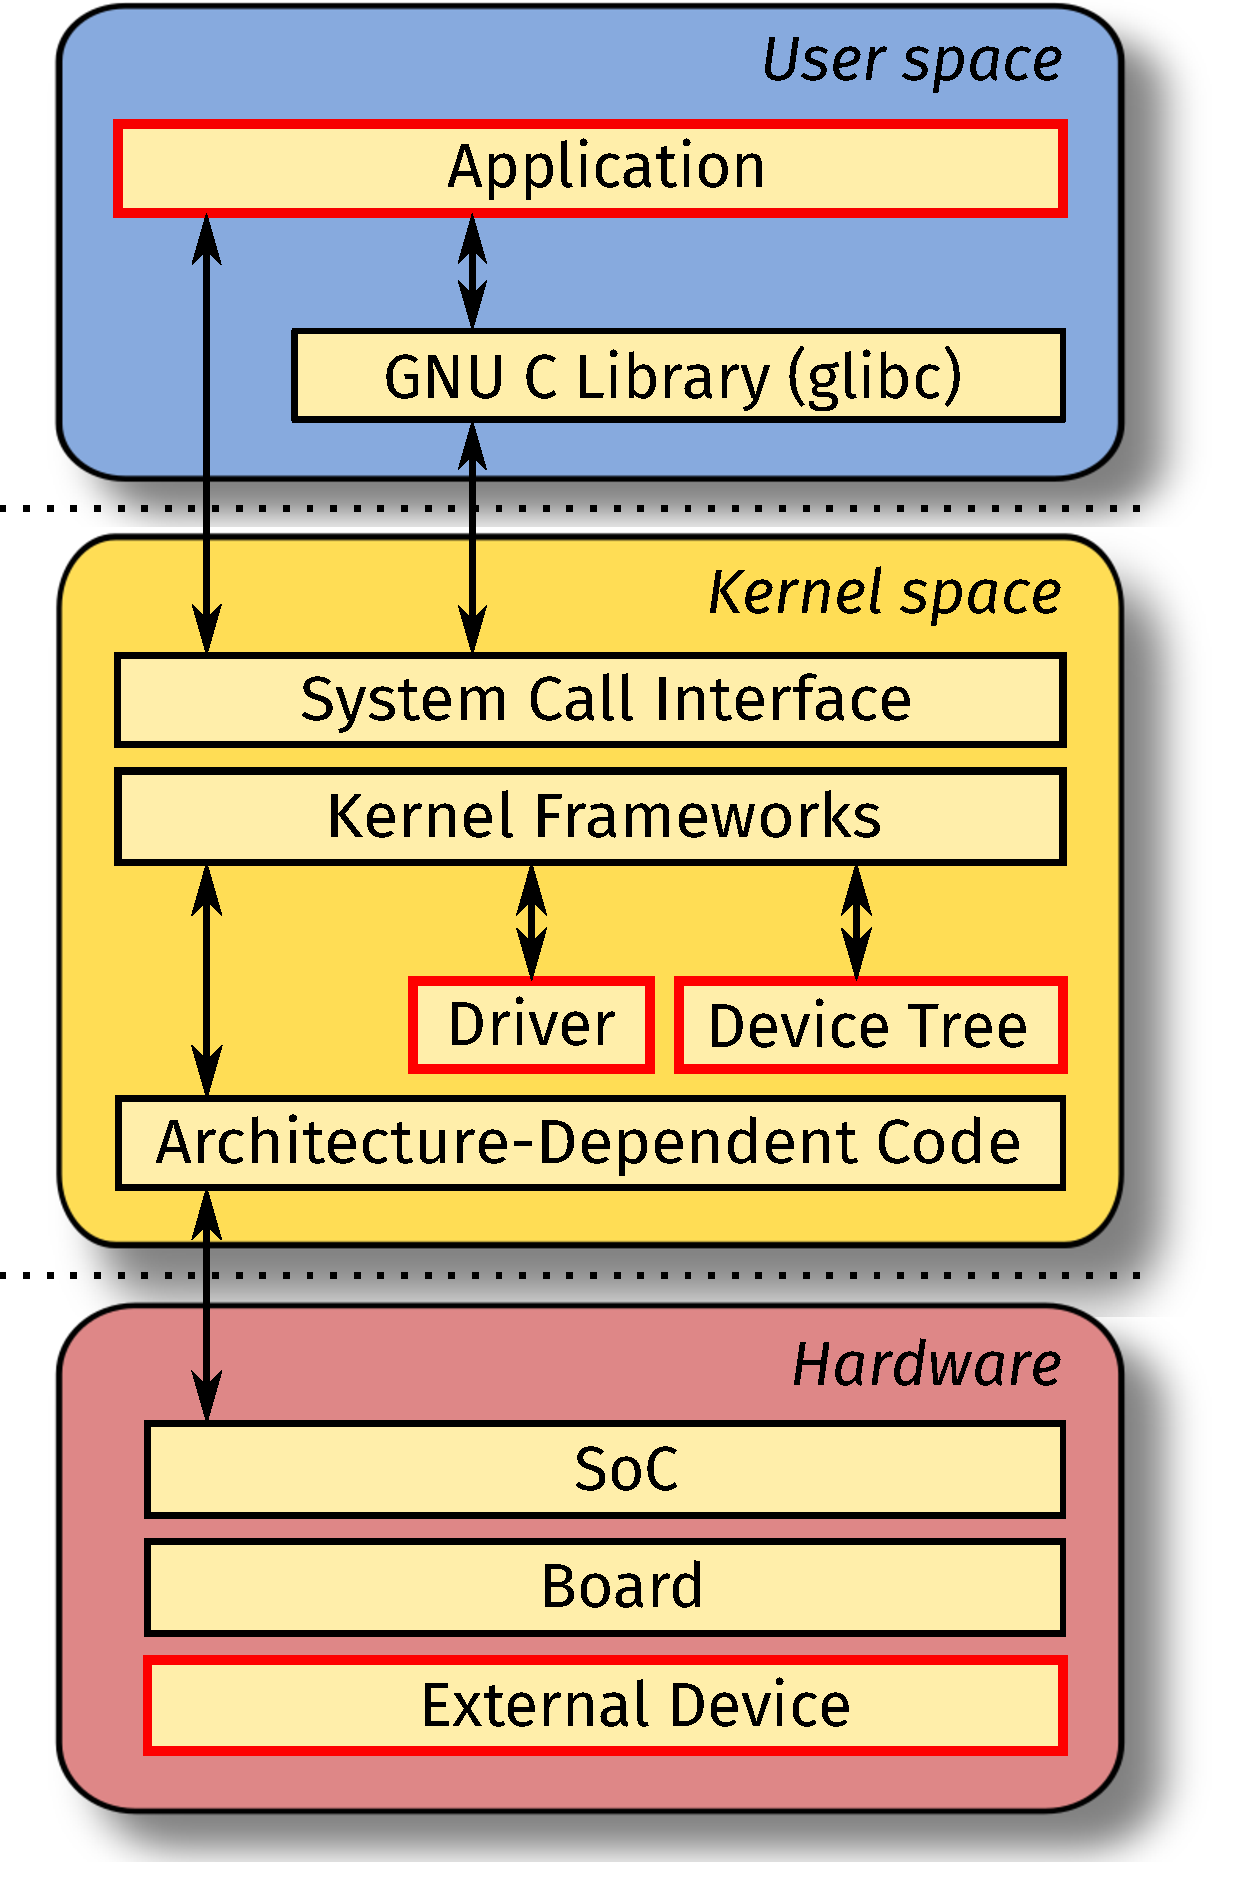
\includegraphics[scale=0.23]{images/architecture.pdf}
  \end{figure}
  \vspace*{-12mm}
\end{frame}

\begin{frame}
  \frametitle{Device Functional Block Diagram}
  \vspace*{-5mm}
  \begin{figure}
    \centering
    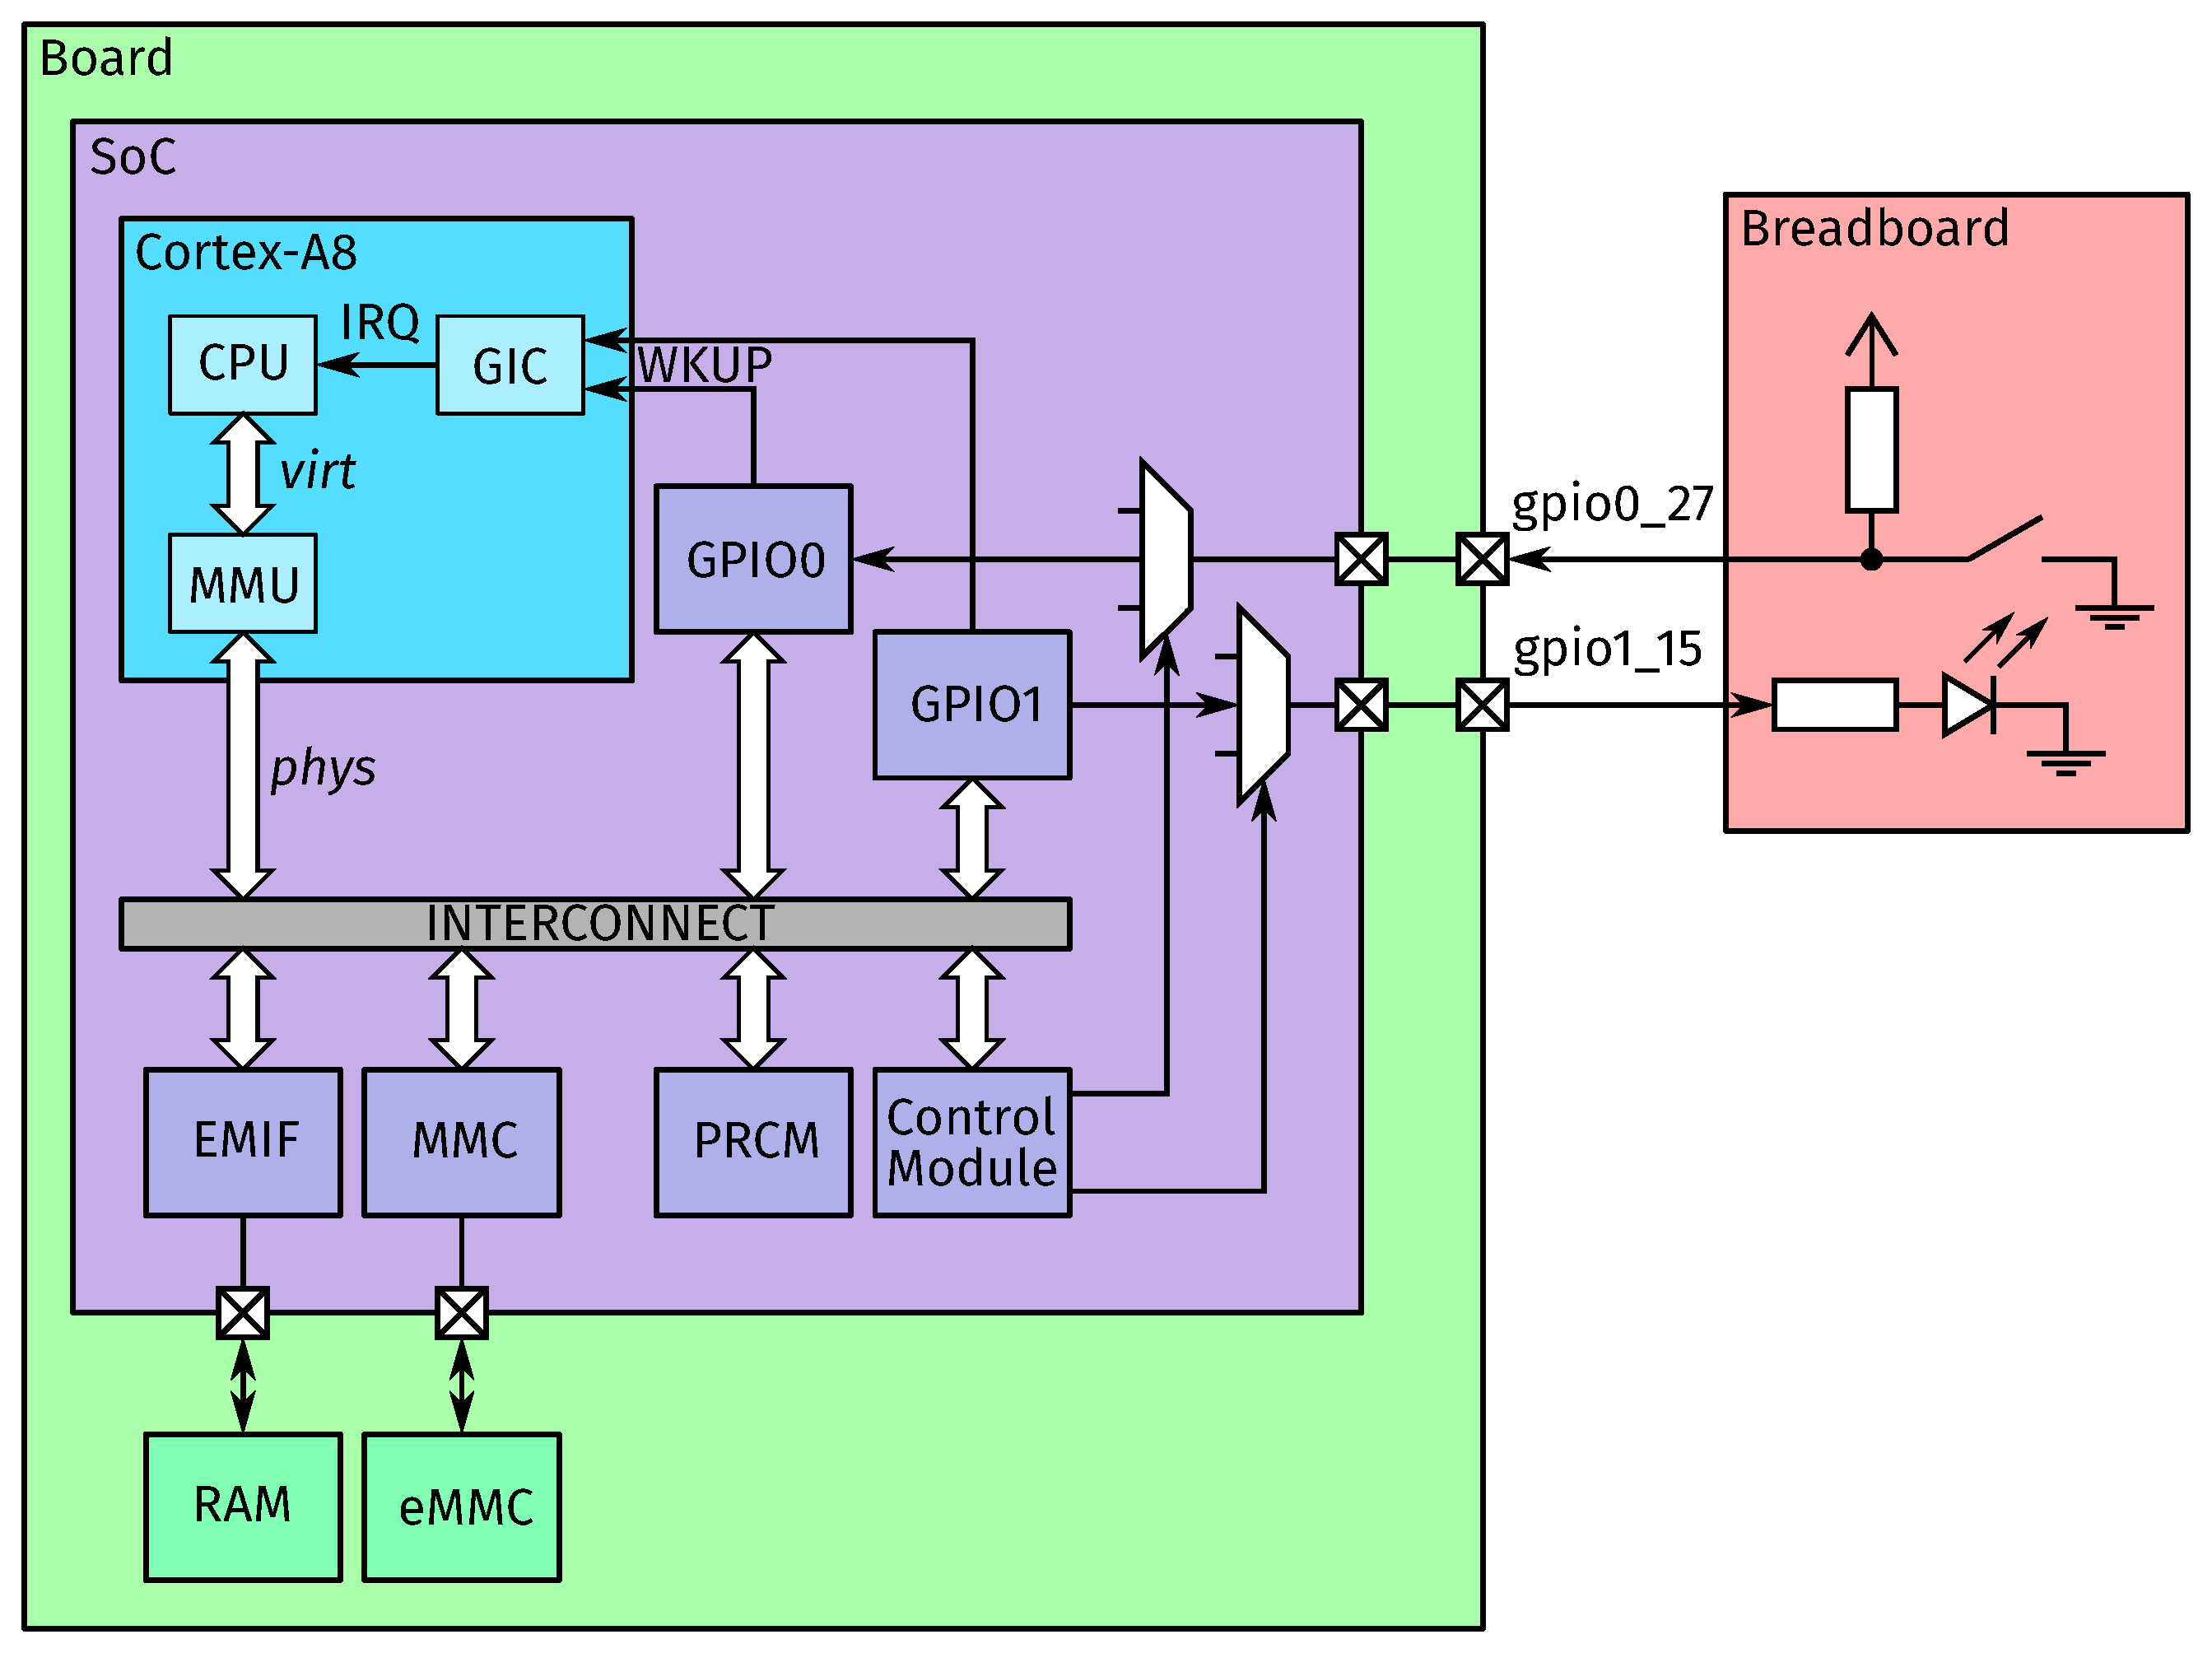
\includegraphics[scale=0.22]{images/architecture2.pdf}
  \end{figure}
  \vspace*{-12mm}
\end{frame}

\section{Hardware Overview}

\subsection{GPIO Module}

\begin{frame}[standout]
  GPIO Module
\end{frame}

\begin{frame}
  \frametitle{Generic GPIO Block}
  \begin{overlayarea}{\textwidth}{\textheight}
    \begin{figure}
      \centering
      \only<1>
      {%
      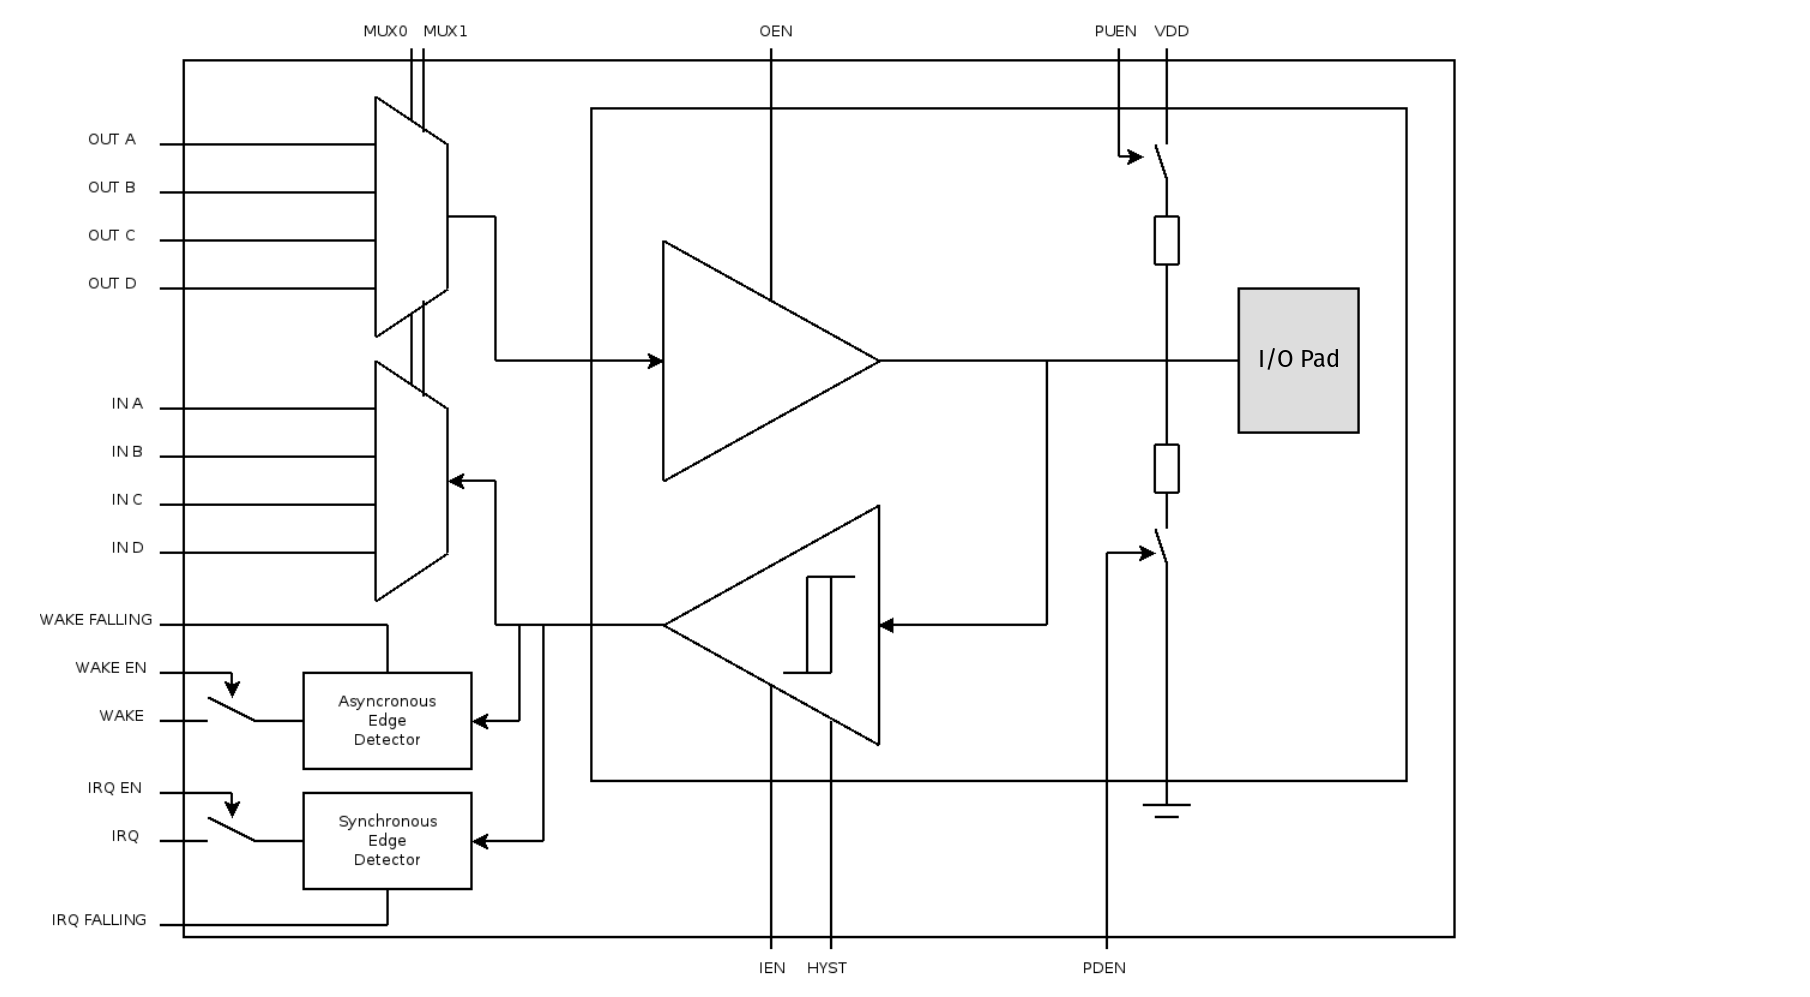
\includegraphics[scale=0.28]{images/gpio-block.png}%
      }%
      \only<2>
      {%
      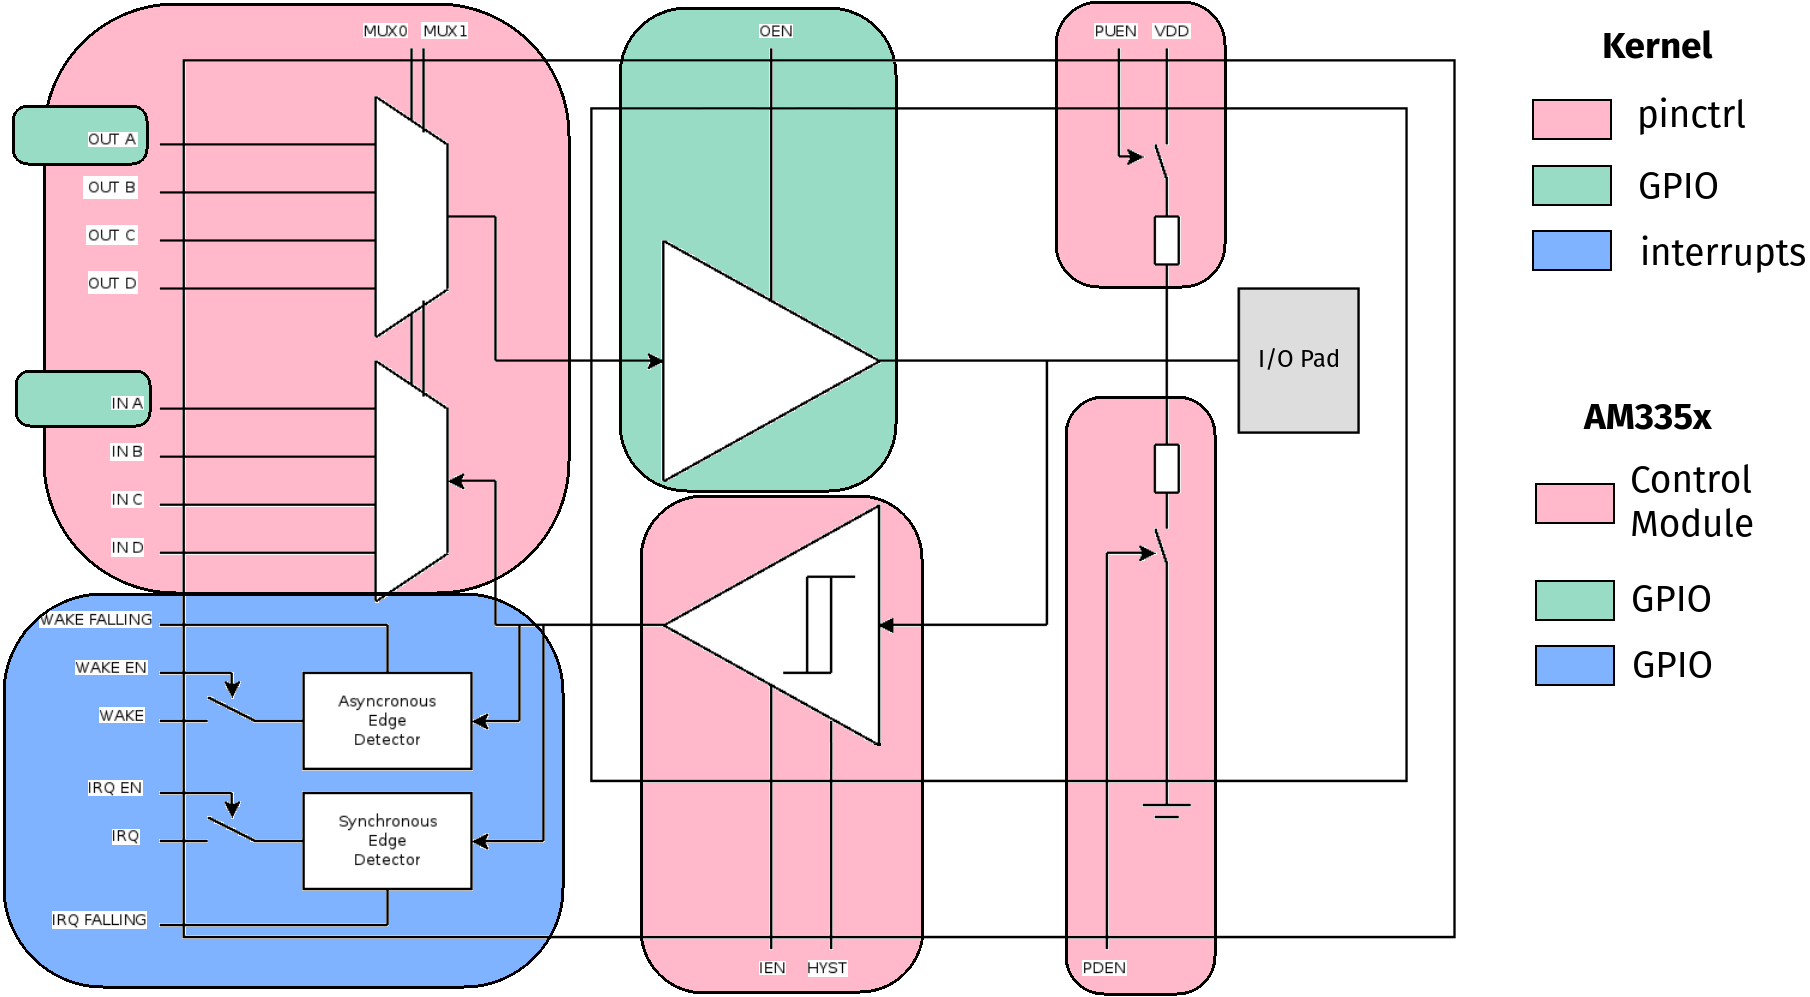
\includegraphics[scale=0.28]{images/gpio-block-color.png}%
      }%
    \end{figure}
  \end{overlayarea}
  \vspace*{-10mm}
\end{frame}

\begin{frame}
  \frametitle{Output Buffers}
  \begin{columns}
    \column{0.5\textwidth}
      \vspace*{-2mm}
      \begin{figure}
        \centering
        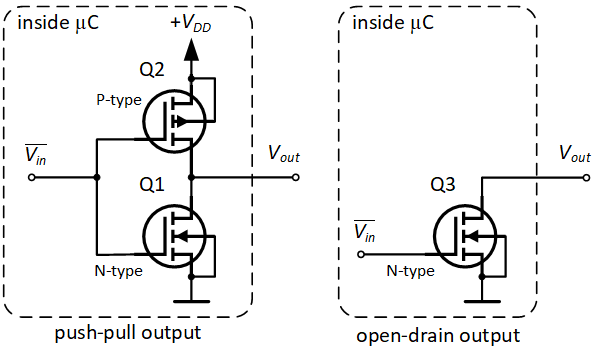
\includegraphics[scale=5]{images/outputs.png}
      \end{figure}
      \vspace*{-5mm}
      \begin{figure}
        \centering
        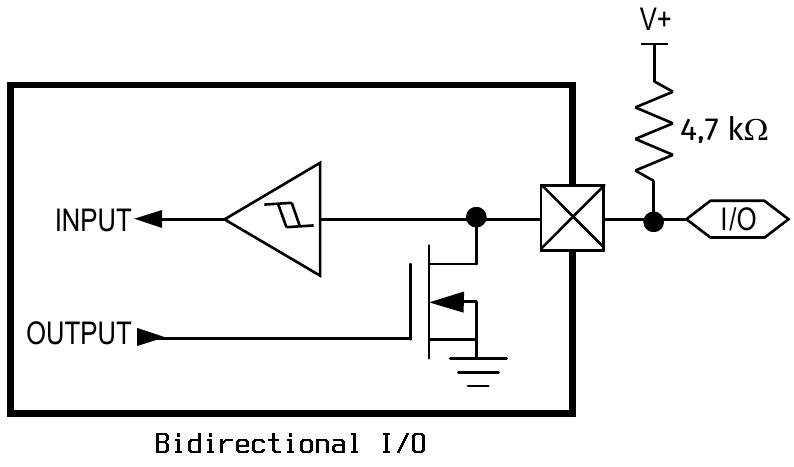
\includegraphics[scale=0.25]{images/open-drain-io.png}
      \end{figure}
      \vspace*{-10mm}
    \column{0.5\textwidth}
      \begin{itemize}
        \item \underline{Push-pull states}: \textbf{0} and \textbf{1}
        \item \underline {Open-drain states}: \textbf{0} and \textbf{Hi-Z}
        \item Open-drain can be bidirectional
        \item External \textbf{pull-up} is usually used
        \item Allows several devices (line sharing, \textbf{wired-AND})
        \item Often used for 1-wire or I2C (bit-banged)
        \item Different voltage can be used
      \end{itemize}
  \end{columns}
\end{frame}

\begin{frame}
  \frametitle{Open-Drain Outputs in AM335x}
  \begin{columns}
    \column{0.5\textwidth}
      \begin{itemize}
        \item In AM335x we don't have \textbf{open-drain outputs}
        \item All GPIO output buffers are push-pull
        \item But we can emulate open-drain output behavior by
              \alert{switching input/output modes}
      \end{itemize}
    \column{0.5\textwidth}
      \textbf{\underline{Push-Pull Output}:}
      \begin{itemize}
        \item \texttt{GPIO\_OE[n] = 0} (fixed, output)
        \item \texttt{GPIO\_DATAOUT[n]:}
        \begin{itemize}
          \item 0: low state
          \item 1: high state
        \end{itemize}
      \end{itemize}
      \textbf{\underline{Open-Drain Output}:}
      \begin{itemize}
        \item \texttt{GPIO\_DATAOUT[n] = 0} (fixed)
        \item \texttt{\textcolor{red}{GPIO\_OE[n]}}:
        \begin{itemize}
          \item 0 (output): low state
          \item 1 (input): Hi-Z state
        \end{itemize}
      \end{itemize}
  \end{columns}
\end{frame}

\begin{frame}
  \frametitle{PRCM: Clock for GPIO}
    \begin{figure}
      \centering
      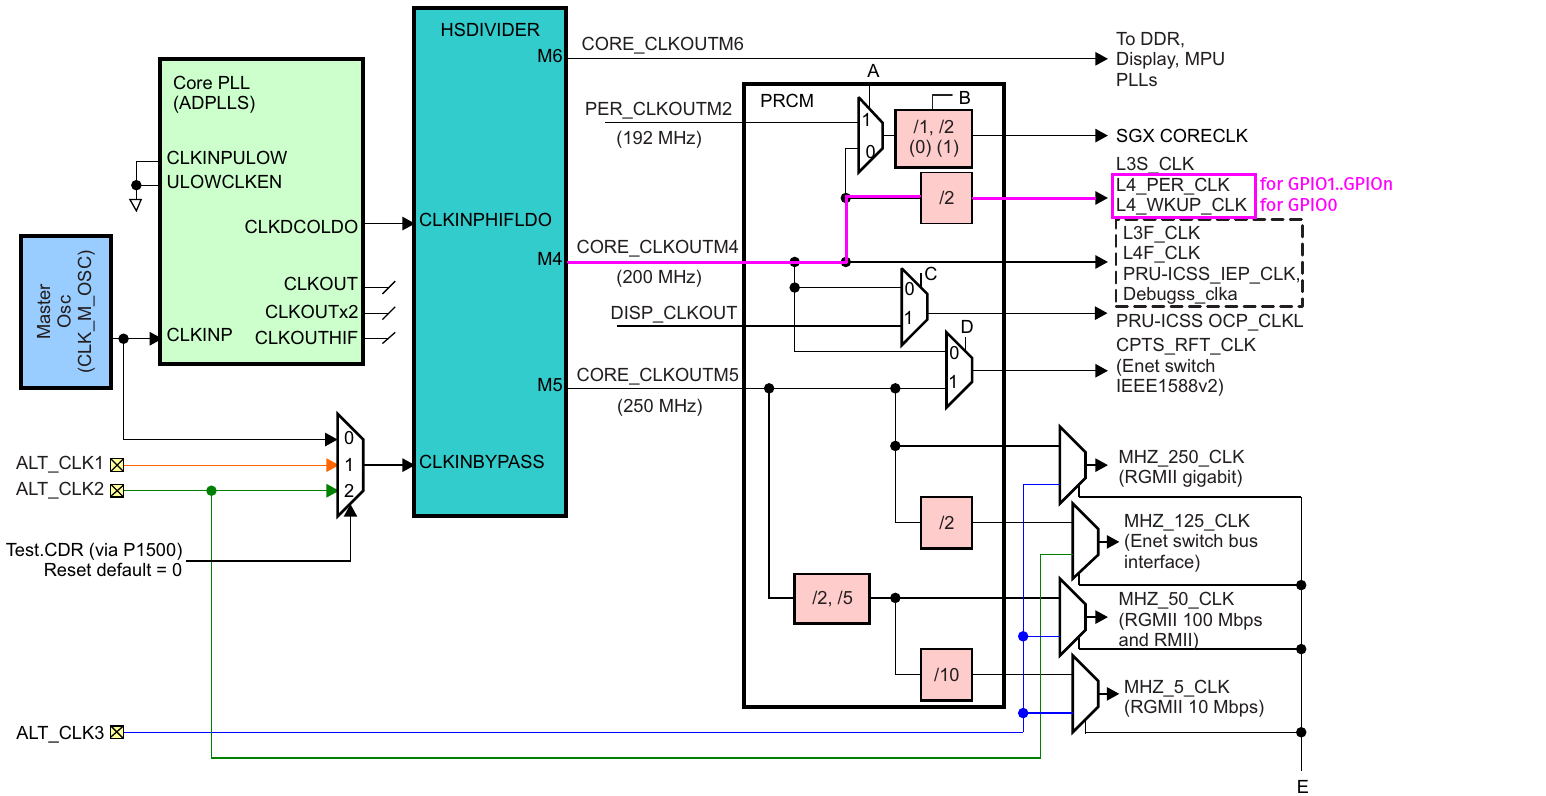
\includegraphics[scale=0.3]{images/dpll-gpio.png}
      \caption{GPIO interface clock derivation}
  \end{figure}
  \vspace*{-12mm}
\end{frame}

\begin{frame}
  \frametitle{Clock Handling inside GPIO}
    \begin{figure}
      \centering
      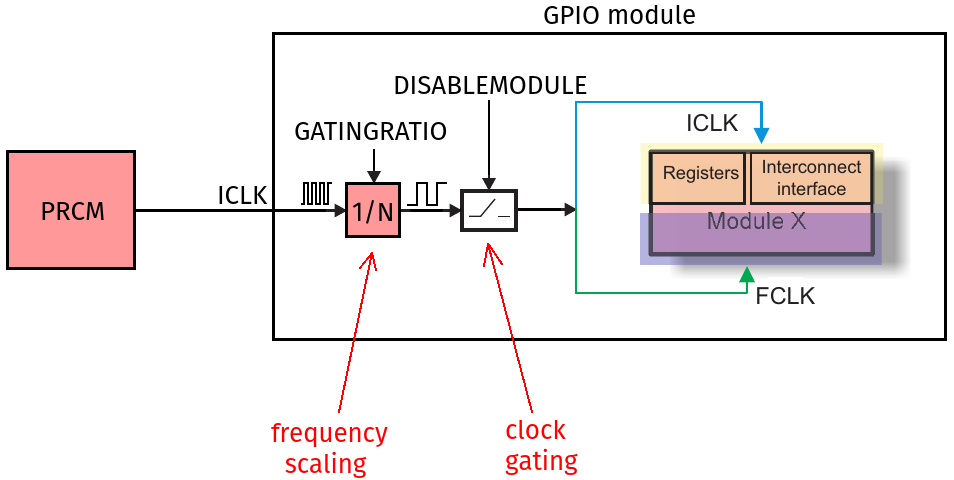
\includegraphics[scale=0.3]{images/gpio-clock.png}
      \caption{Clock path inside of GPIO module}
  \end{figure}
  \[ P \approx P_{dyn} = C \cdot f \cdot V^2 \]
\end{frame}

\begin{frame}
  \frametitle{Power Management Consideration}
  \begin{overlayarea}{\textwidth}{\textheight}
    \begin{figure}
      \centering
      \only<1>
      {%
      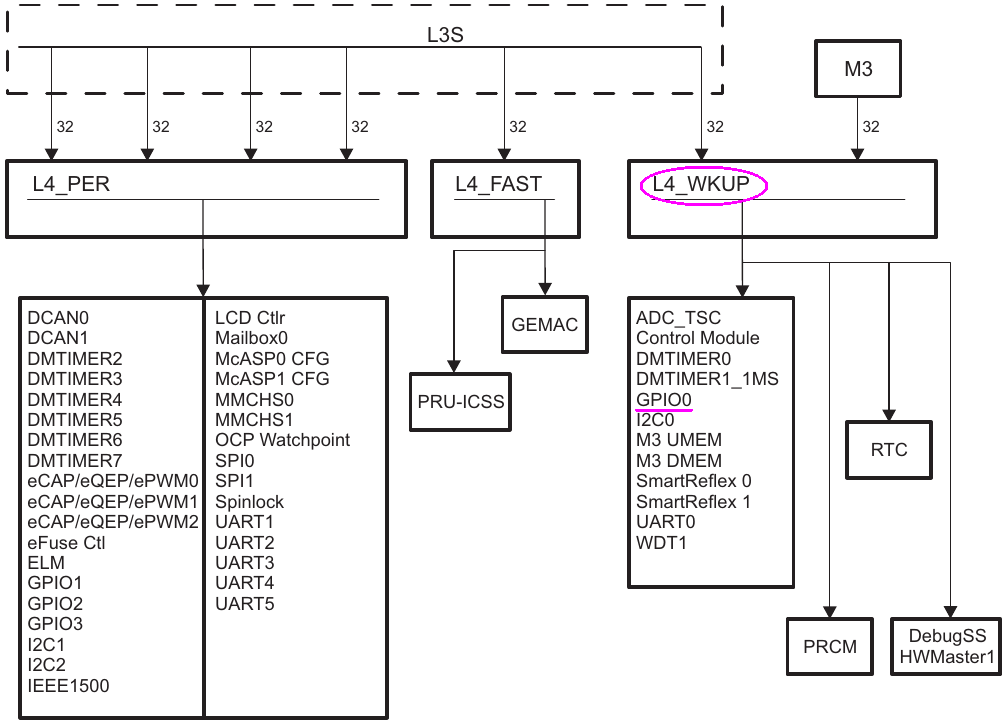
\includegraphics[scale=0.3]{images/l4-gpio0-wkup.png}
      }%
      \only<2>
      {%
      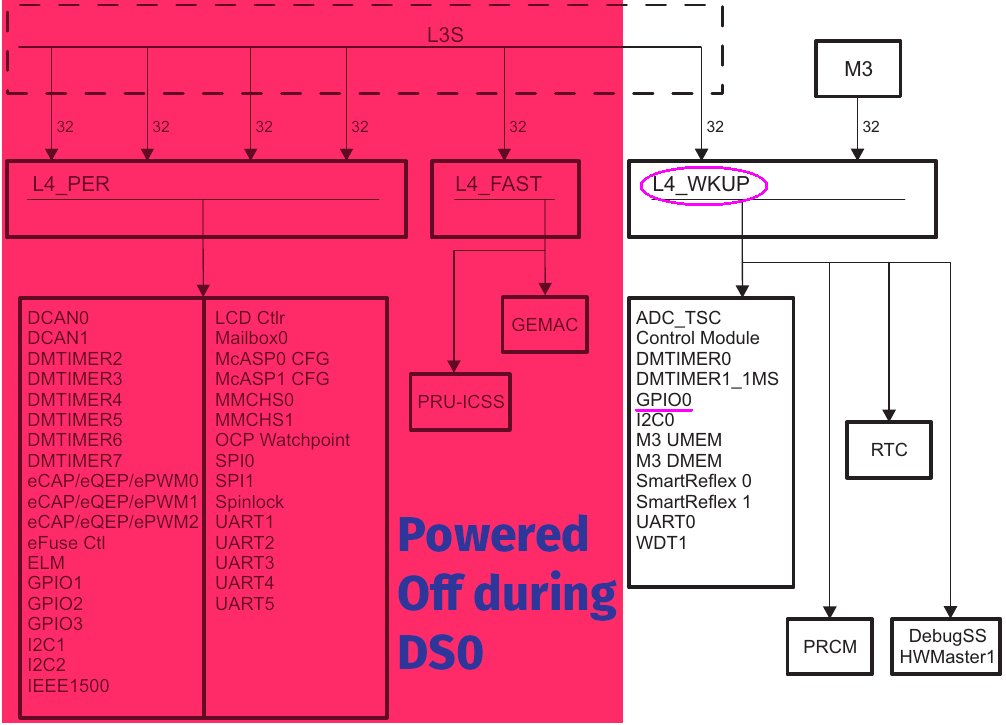
\includegraphics[scale=0.3]{images/l4-gpio0-wkup-ds0.png}
      }%
      \caption{L4 Topology (Figure 10-2 in TRM)}
    \end{figure}
  \end{overlayarea}
  \vspace*{-10mm}
\end{frame}

\begin{frame}
  \frametitle{Debouncing}
  \begin{overlayarea}{\textwidth}{.8\textheight}
    \begin{figure}
      \centering
      \only<1>
      {%
      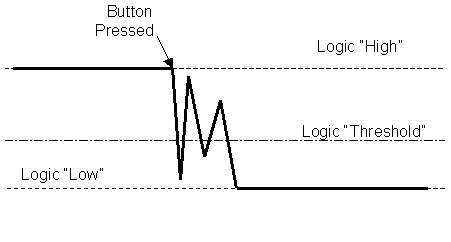
\includegraphics[scale=0.6]{images/debouncing1.png}
      }%
      \only<2>
      {%
      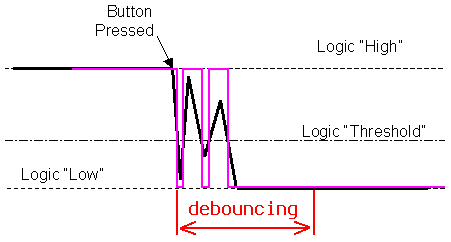
\includegraphics[scale=0.6]{images/debouncing2.png}
      }%
      \caption{Button Debouncing}
    \end{figure}
  \end{overlayarea}
\end{frame}

\begin{frame}
  \frametitle{Debouncing (cont'd)}
  \begin{itemize}
    \item Debouncing: software or hardware
    \item AM335x has GPIO debouncing capability:
    \begin{itemize}
      \item \texttt{GPIO\_DEBOUNCEENABLE[31:0]}
      \item \texttt{GPIO\_DEBOUNCINGTIME[7:0]}
    \end{itemize}
    \item Kernel API:
    \begin{itemize}
      \item Old: \texttt{gpio\_set\_debounce()}
      \item New: \texttt{gpiod\_set\_debounce()}
    \end{itemize}
  \end{itemize}
\end{frame}

\subsection{Choosing Pins}

\begin{frame}[standout]
  Choosing Pins
\end{frame}

\begin{frame}
  \frametitle{BBB Expansion Headers}
  \begin{figure}
    \centering
    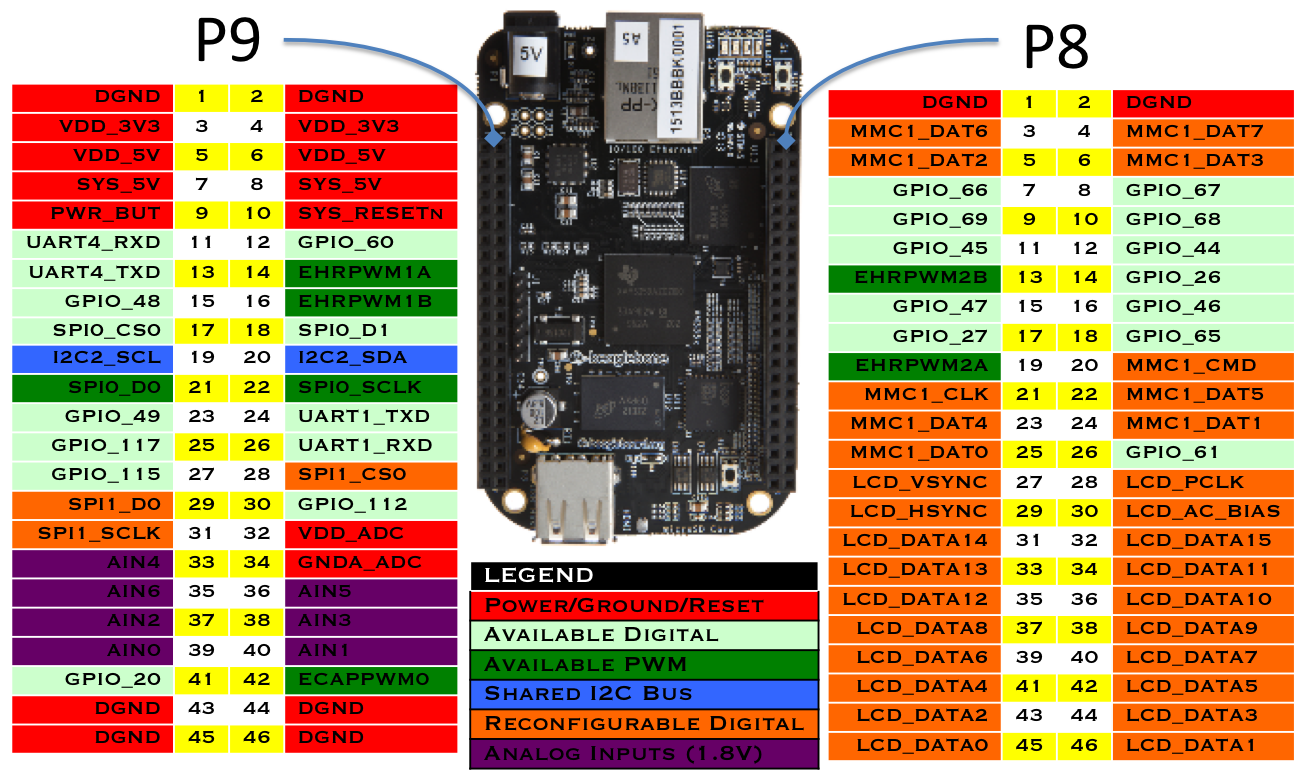
\includegraphics[scale=0.29]{images/expansion-headers.png}
    \caption{BBB Cape Expansion Headers}
  \end{figure}
  \vspace*{-10mm}
\end{frame}

\begin{frame}
  \frametitle{Choosing GPIO Pins}
  \begin{figure}
    \centering
    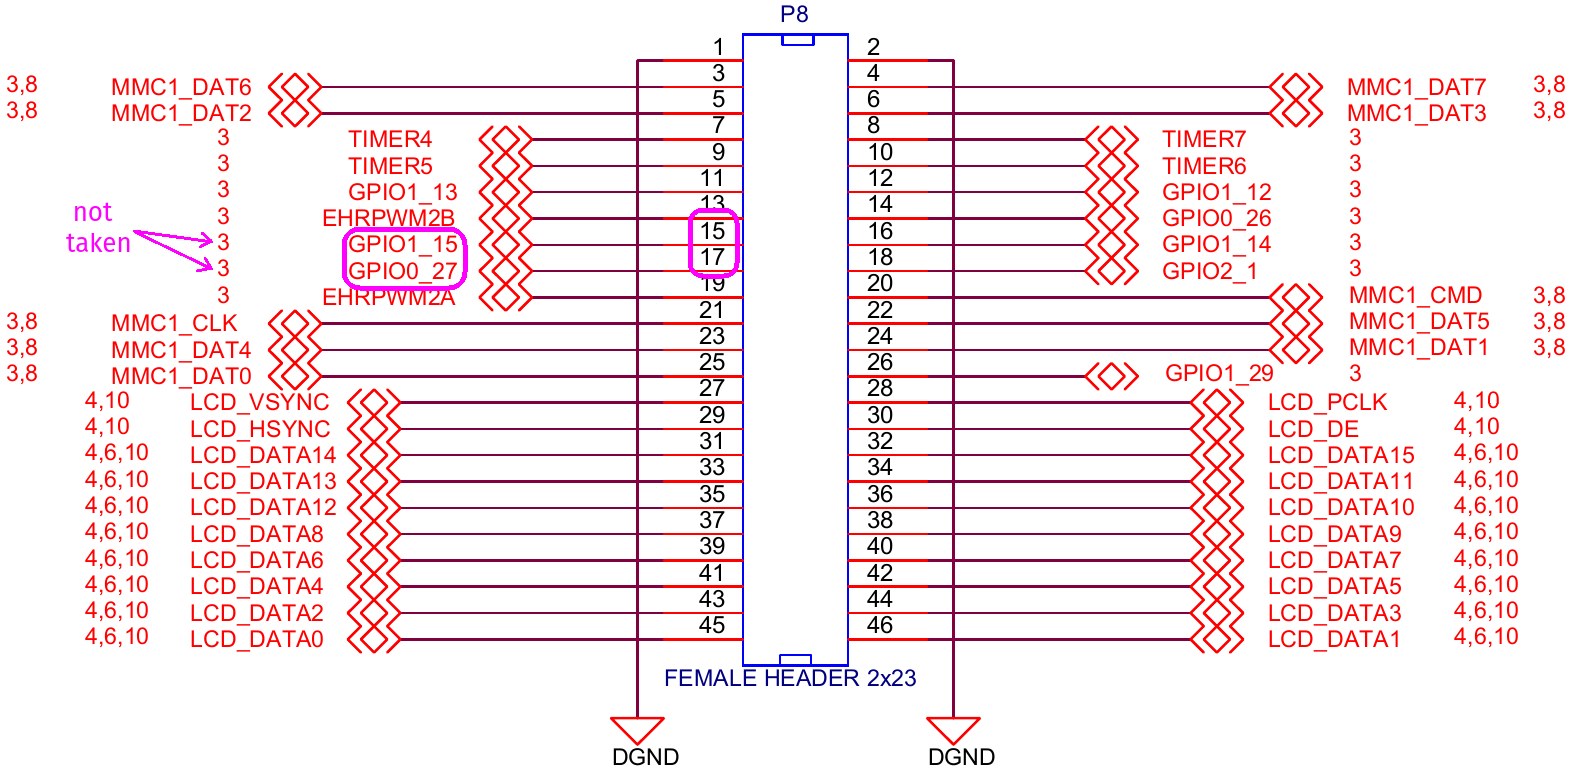
\includegraphics[scale=0.29]{images/p8.png}
    \caption{P8 Expansion Header}
  \end{figure}
  \vspace*{-10mm}
\end{frame}

\begin{frame}
  \frametitle{Choosing GPIO Pins (cont'd)}
  \begin{figure}
    \centering
    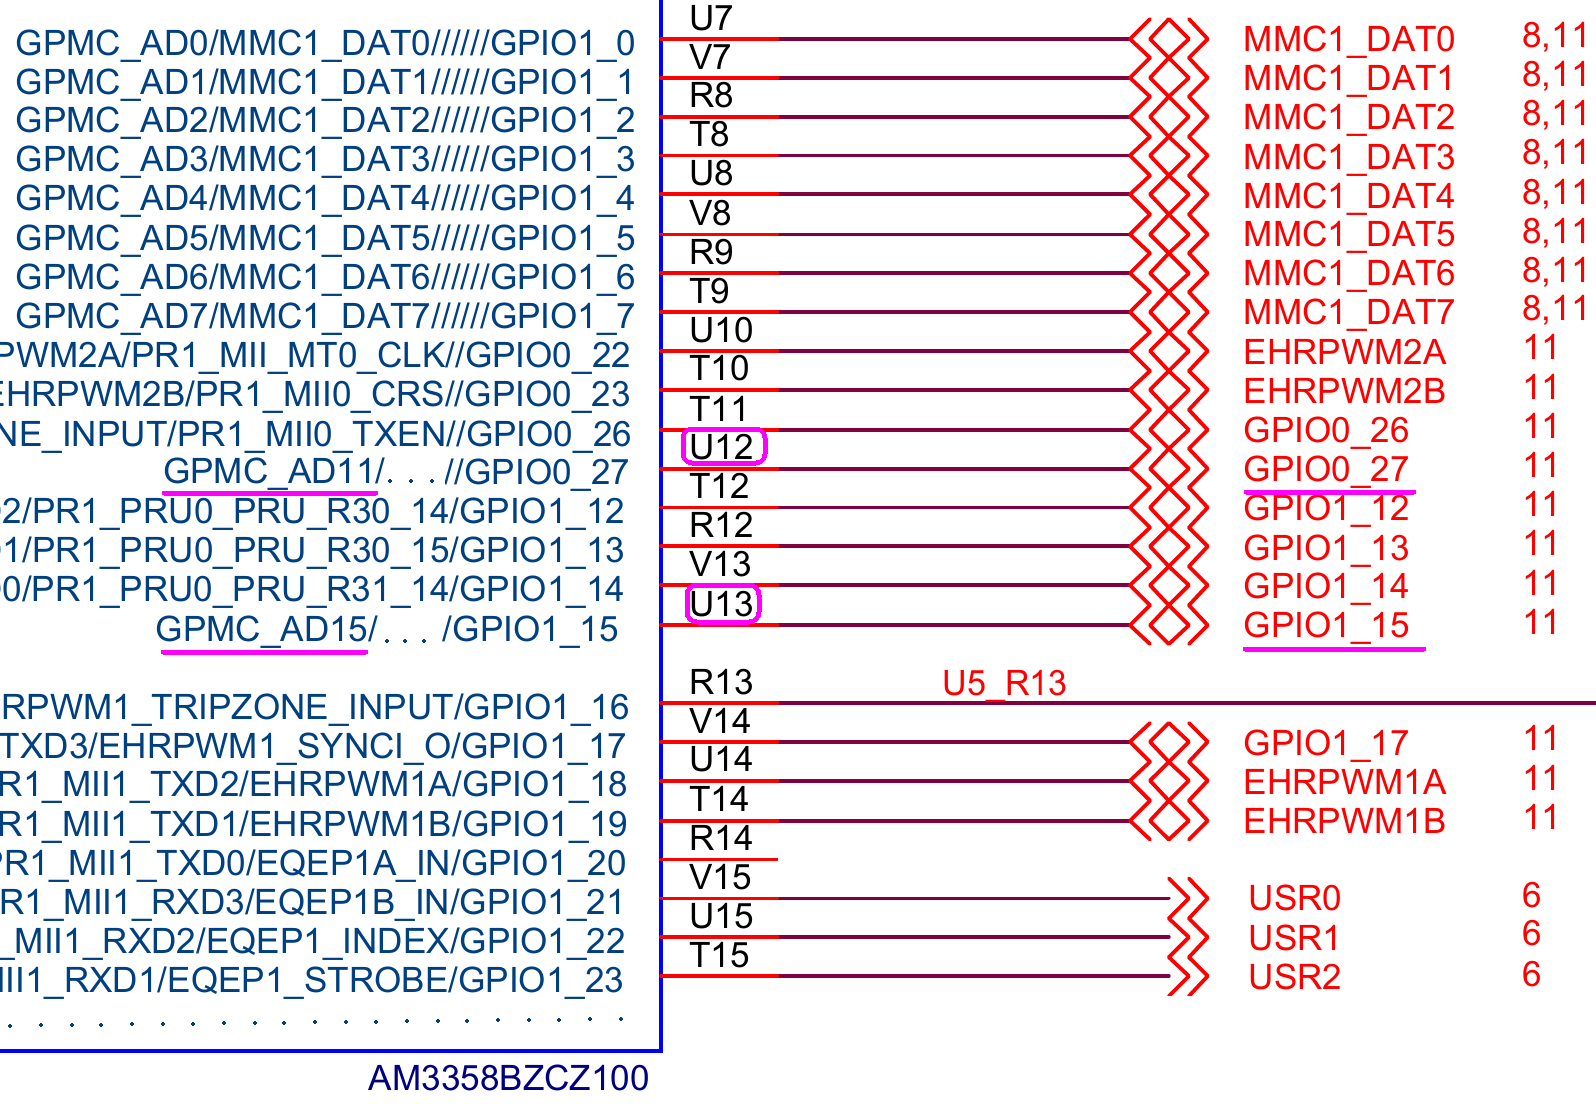
\includegraphics[scale=0.2]{images/soc-pins.png}
    \caption{AM3358 pins}
  \end{figure}
  \vspace*{-10mm}
\end{frame}

\subsection{Registers and Values}

\begin{frame}[standout]
  Registers and Values
\end{frame}

\begin{frame}
  \frametitle{Pin Multiplexing}
  \begin{figure}
    \centering
    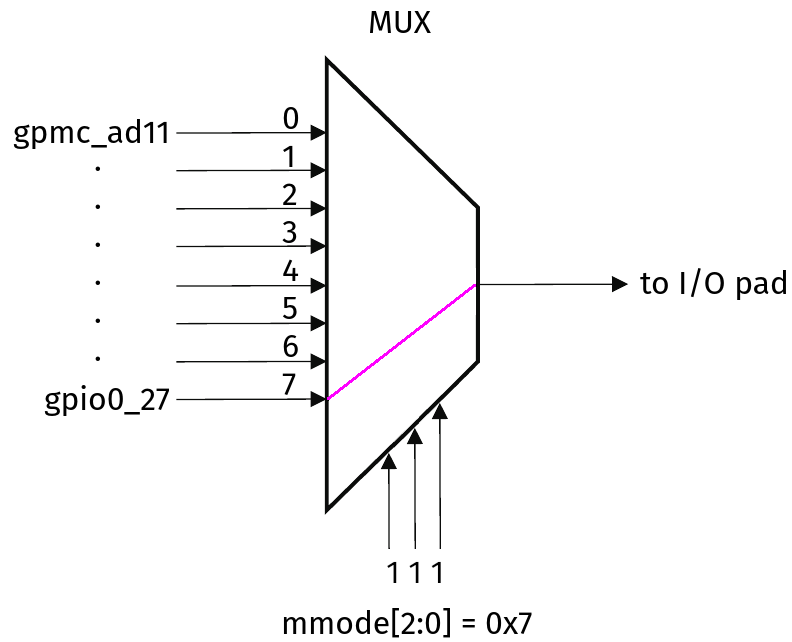
\includegraphics[scale=0.3]{images/mux.png}
    \caption{Pin mux example}
  \end{figure}
\end{frame}

\begin{frame}
  \frametitle{Pin Modes}
    \begin{figure}
      \centering
      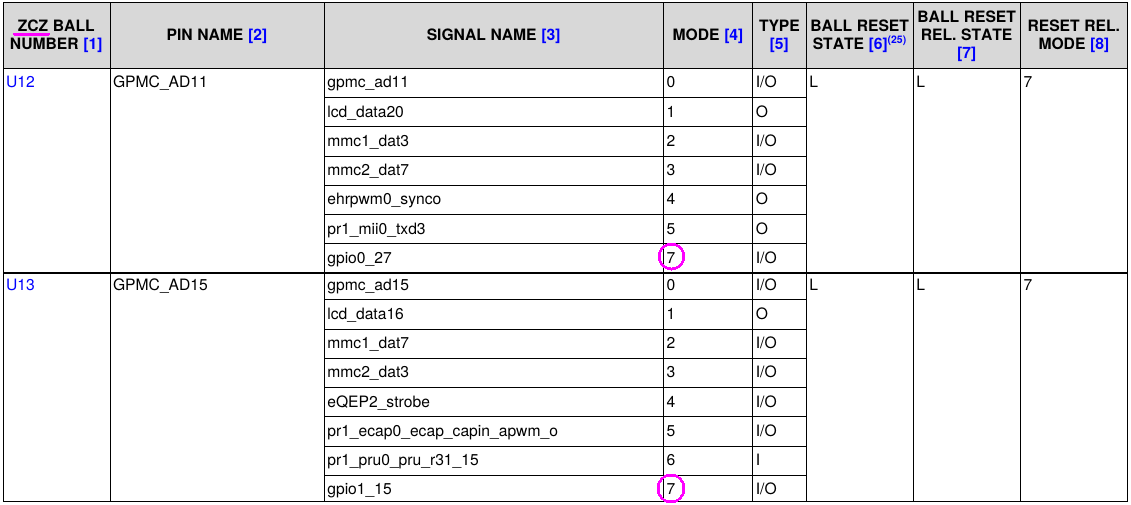
\includegraphics[scale=0.4]{images/pin-modes.png}
      \caption{Pin attributes (Table 4-2 in datasheet)}
  \end{figure}
  \vspace*{-10mm}
\end{frame}

\begin{frame}
  \frametitle{Modules Addresses}
    \begin{figure}
      \centering
      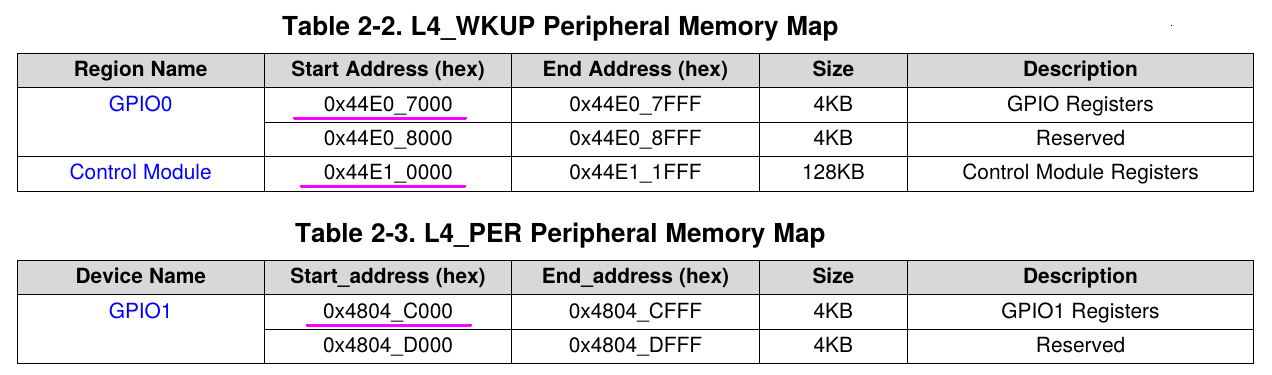
\includegraphics[scale=0.3]{images/regs-base.png}
      \caption{Base addresses of registers (``Memory Map'' section)}
  \end{figure}
\end{frame}

\begin{frame}
  \frametitle{Pin Control Registers}
    \begin{figure}
      \centering
      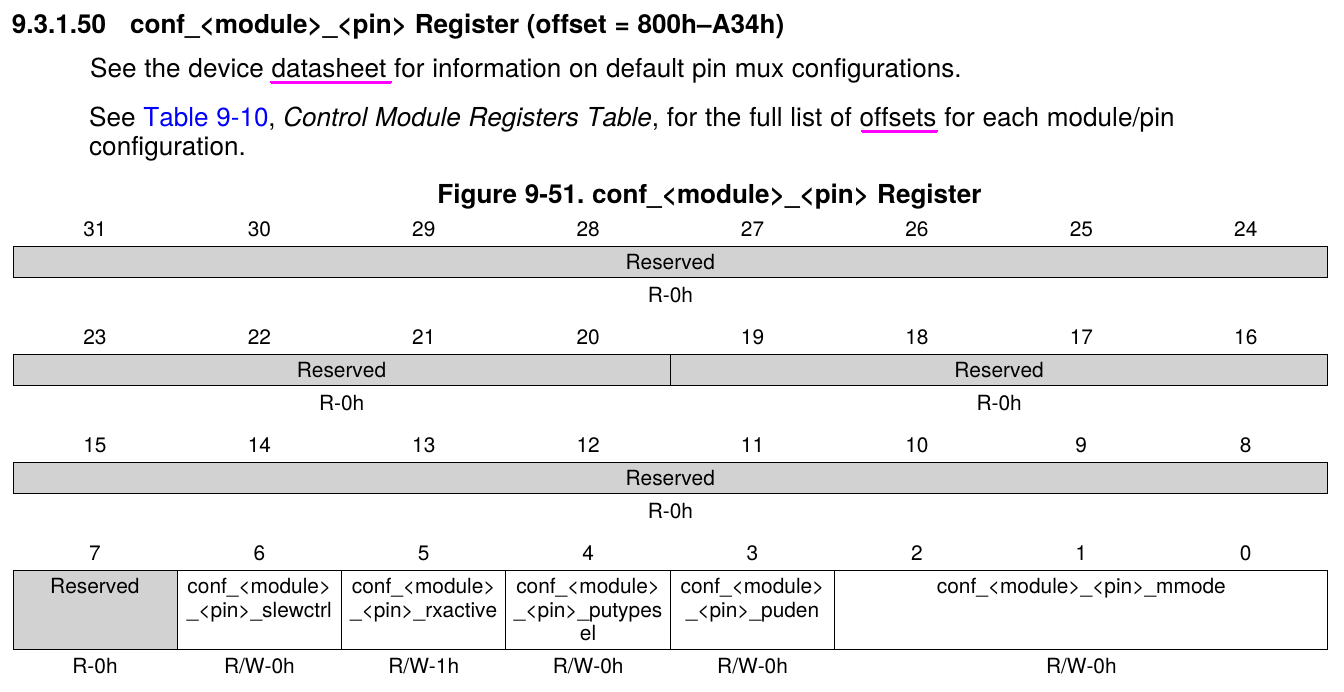
\includegraphics[scale=0.3]{images/conf-reg.png}
      \caption{Pin mux registers description (``Control Module'' section)}
  \end{figure}
  \vspace*{-10mm}
\end{frame}

\begin{frame}
  \frametitle{Pin Control Registers (cont'd)}
    \begin{figure}
      \centering
      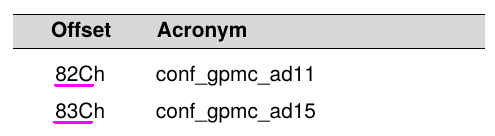
\includegraphics[scale=0.5]{images/conf-offsets.png}
      \caption{Pin mux registers offsets (``Control Module'' section)}
  \end{figure}
\end{frame}

\begin{frame}
  \frametitle{GPIO Registers Offset}
    \begin{figure}
      \centering
      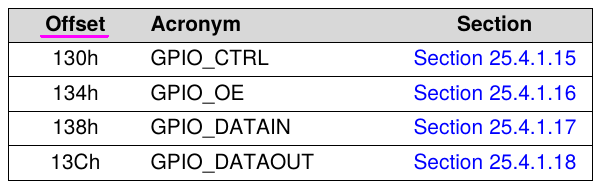
\includegraphics[scale=0.5]{images/gpio-registers-offset.png}
      \caption{Address offset for GPIO registers}
  \end{figure}
\end{frame}

\begin{frame}
  \frametitle{GPIO\_CTRL Register}
    \begin{figure}
      \centering
      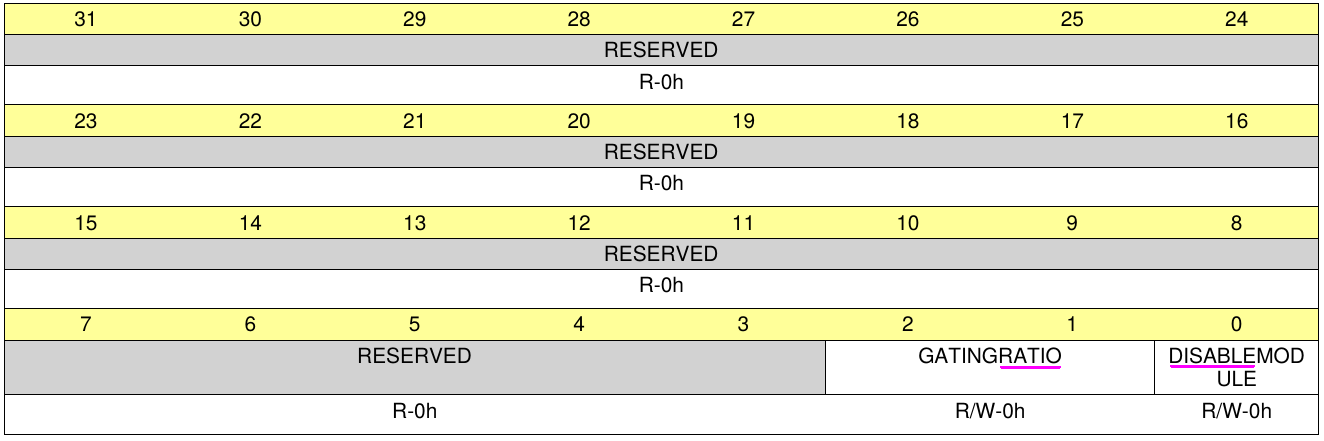
\includegraphics[scale=0.3]{images/gpio-ctrl.png}
      \caption{GPIO\_CTRL register}
  \end{figure}
\end{frame}

\begin{frame}
  \frametitle{Rest of GPIO Registers}
    \begin{figure}
      \centering
      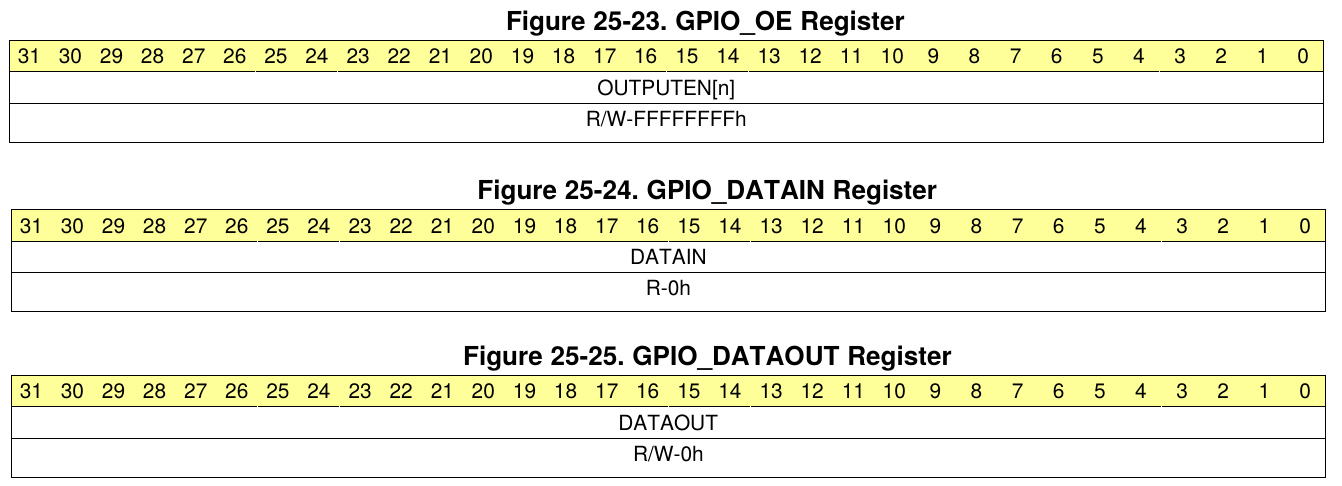
\includegraphics[scale=0.3]{images/gpio-common-regs.png}
      \caption{GPIO common registers}
  \end{figure}
\end{frame}

\begin{frame}[standout]
  Take five
\end{frame}

\subsection{Building the Device}

\begin{frame}[standout]
  Building the Device
\end{frame}

\begin{frame}
  \frametitle{Interfacing LED}
  \begin{columns}
    \column{0.5\textwidth}
      \scalebox{0.8} {
      \begin{circuitikz}[scale=1]
      \draw[darkgreen, thick]
        (0,4) to [battery1, l_=$V_s$] (0,0)
        (0,4) to [R, l=$R$, a=$\SI{330}{\ohm}$, i=$I_f$] (4,4)
        (4,4) to [leDo, v=$V_f$] (4,0)
        (4,0) to [short] (0,0)
        ;
        \draw (4.2,2.5) node[right,color=black]{$D$};
        \draw (0,2.3)   node[right,color=black]{$+$};
      \end{circuitikz}
      }
    \column{0.5\textwidth}
      \hspace*{5mm}
      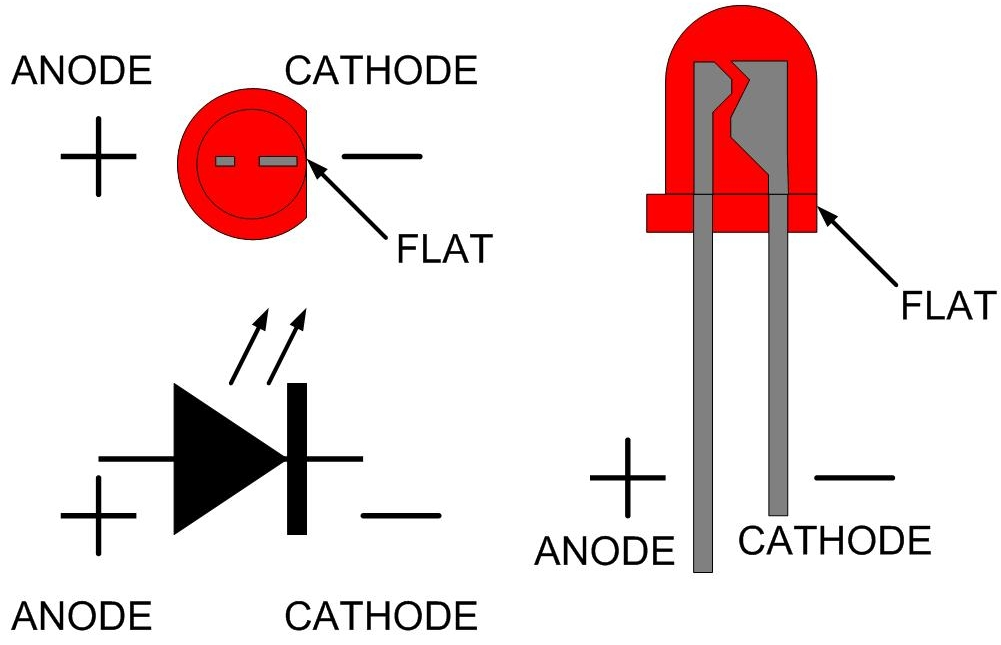
\includegraphics[scale=0.2]{images/ledwiring.jpg}
  \end{columns}

  \begin{columns}
    \column{0.5\textwidth}
      \begin{flalign*}
        & V_s = \SI{3.3}{\volt}             && \text{(BBB GPIO voltage)}    & \\
        & V_f = \SI{2.0}{\volt}             && \text{(for red LED)}         & \\
        & I_{LED}  = \SI{20}{\milli\ampere} && \text{(nominal LED current)} & \\
        & I_{GPIO} = \SI{4}{\milli\ampere}  && \text{(max BBB GPIO)} &
      \end{flalign*}
    \column{0.5\textwidth}
      \begin{alignat*}{3}
        & R = \frac{V_s - V_f}{I_f}                           & \\
        & R = \frac{3.3 - 2.0}{0.004} \approx \SI{330}{\ohm}  &
      \end{alignat*}
  \end{columns}
  \vspace*{-5mm}
\end{frame}

\begin{frame}
  \frametitle{Interfacing Button}
  \begin{columns}
    \column{0.4\textwidth}
      \scalebox{0.8} {
      \begin{circuitikz}[scale=1]
      \draw[darkgreen, thick]
        (1,0)   to [short, -*] (2.3,0)
                to [R, l=$R$, a=$\SI{10}{\kilo\ohm}$] (2.3,2)
                node[vcc]{$V_{CC}$}
        (2.3,0) to [nos, l=$S$] (5,0)
                to [short] (5,-0.5)
                node[ground]{}
        ;
      \node [pin] at (0.75,0){};
      \draw (0.35,0.5) node[right]{$pin$};
      \end{circuitikz}
      }
      \par \vspace*{5mm} \hspace*{2mm}
      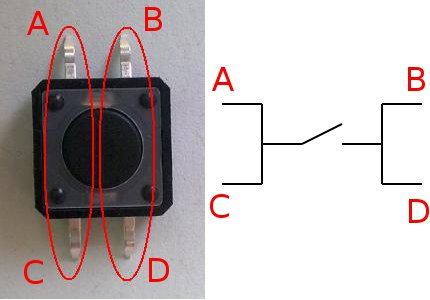
\includegraphics[scale=0.32]{images/pushbutton.jpg}
    \column{0.6\textwidth}
      Logic:
      \begin{itemize}
        \item Button pressed: $V_{pin} = \SI{0}{\volt}$
        \item Button not pressed: $V_{pin} = V_{CC} = \SI{3.3}{\volt}$
      \end{itemize}
      Pull-up resistor:
      \begin{itemize}
        \item Current must be strong enough to eliminate noise
        \item But we don't want too much power to be drawn either
        \item Pull-up resistor is usually $\SI{10}{\kilo\ohm}$
      \end{itemize}
  \end{columns}
\end{frame}

\begin{frame}
  \frametitle{Breadboard}
    \begin{figure}
      \centering
      \begin{overlayarea}{\textwidth}{0.8\textheight}
        \only<1>{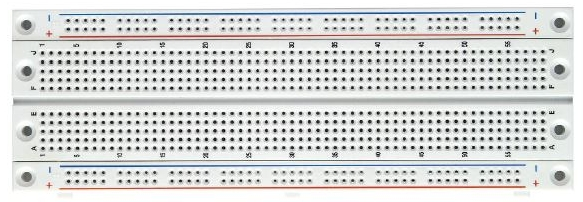
\includegraphics[scale=1.1]{images/eic20020.jpg}}
        \only<2>{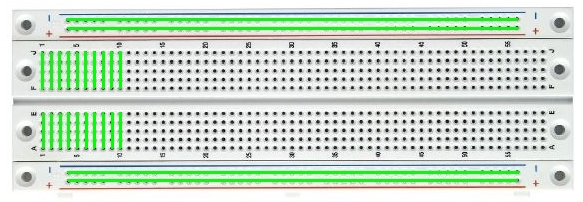
\includegraphics[scale=1.1]{images/eic20020_marked.jpg}}
        \caption{EIC-20020 Breadboard}
      \end{overlayarea}
  \end{figure}
\end{frame}

\begin{frame}
  \frametitle{Device: Schematics}
    \begin{figure}
      \centering
      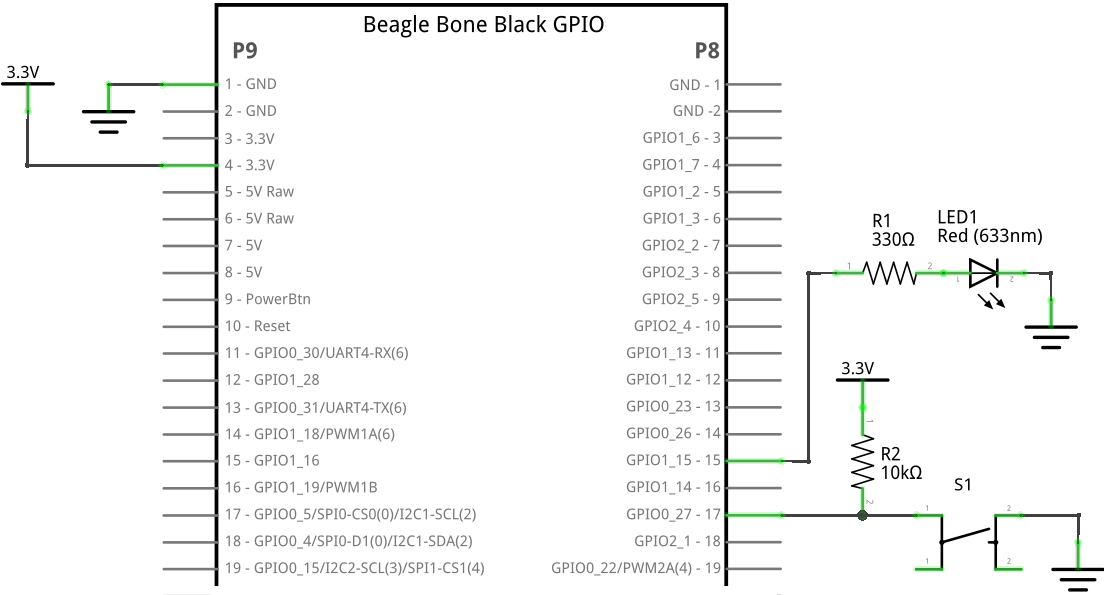
\includegraphics[scale=1]{images/lab1_schem.png}
      \caption{Schematics of device}
  \end{figure}
  \vspace*{-5mm}
\end{frame}

\begin{frame}
  \frametitle{Device: Prototyping}
    \begin{figure}
      \centering
      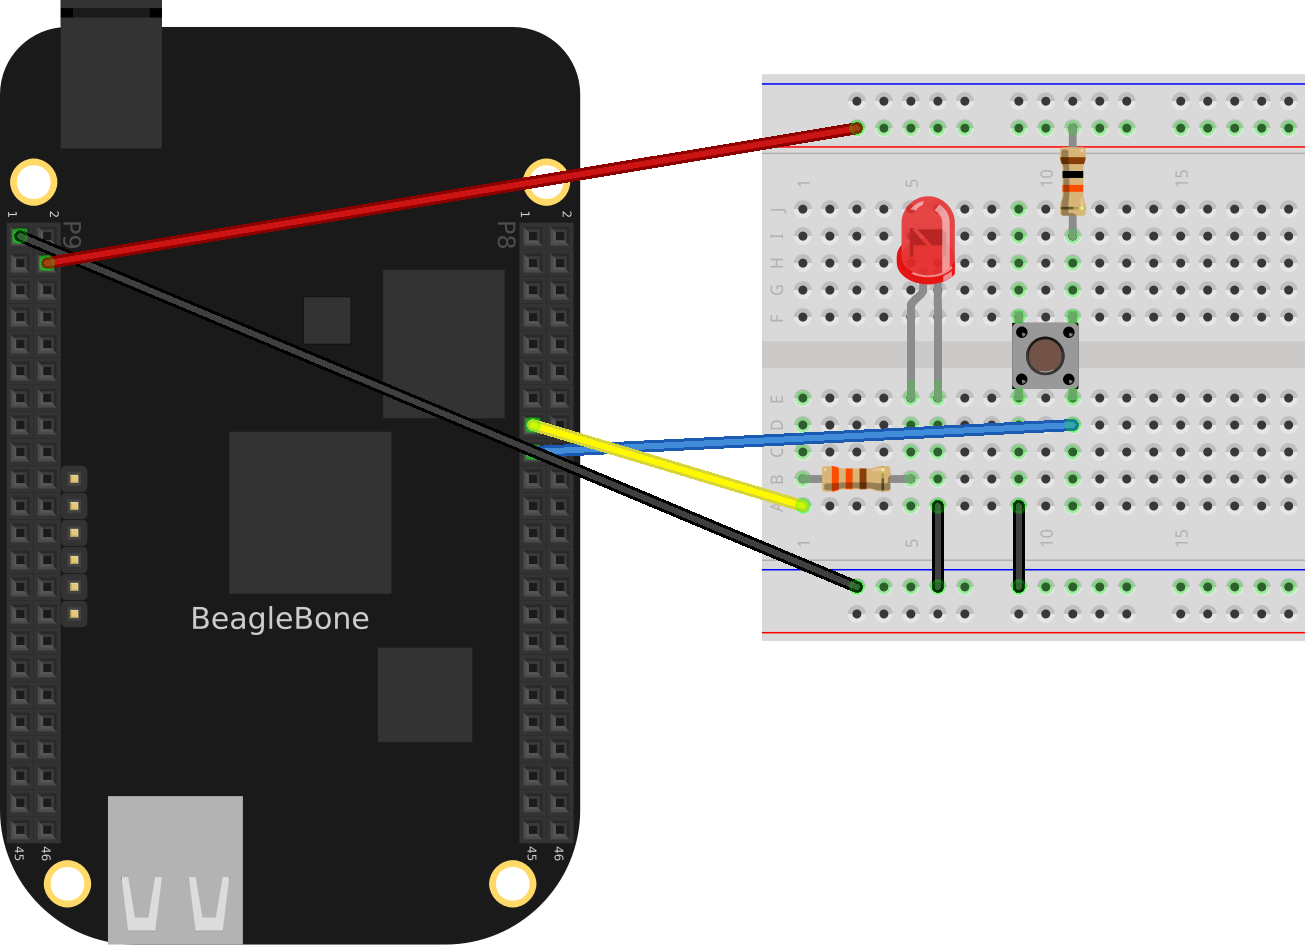
\includegraphics[scale=0.7]{images/lab1_bb.png}
      \caption{Breadboard connections}
  \end{figure}
  \vspace*{-12mm}
\end{frame}

\section{Kernel Driver: Na\"ive Approach}

\subsection{First Attempt}

\begin{frame}[standout]
  \textbf{Attempt \#1} \\
  \vspace{5mm}
  Direct access to registers \\
  \vspace{5mm}
  \alert{DO NOT USE IN REAL LIFE!}
\end{frame}

\begin{frame}[containsverbatim]
  \frametitle{API: ioremap}
  \begin{figure}
    \centering
    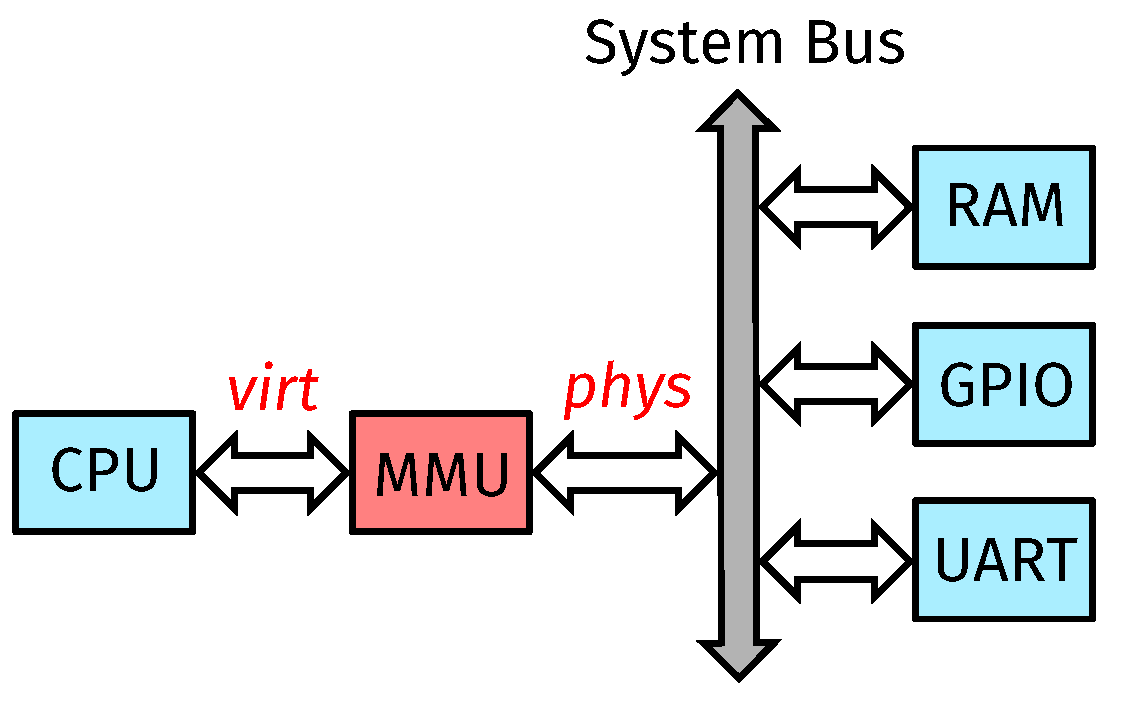
\includegraphics[scale=0.3]{images/phys-virt-ioremap.pdf}
  \end{figure}

  \begin{lstlisting}[language=c,numbers=none]
virt_addr = ioremap(phys_addr, size);
  \end{lstlisting}
\end{frame}

\begin{frame}[containsverbatim]
  \frametitle{API: ioremap (cont'd)}
  \begin{lstlisting}[language=c,numbers=none]
#include <asm/io.h>

/* Create/remove the mapping to virtual address space for I/O region */
void __iomem *ioremap(resource_size_t res_cookie, size_t size);
void iounmap(volatile void __iomem *iomem_cookie);

/* Read/write primitives: handle memory barriers, endianness, volatile */
void iowrite32(u32 value, volatile void __iomem *addr);
u32 ioread32(const volatile void __iomem *addr);
  \end{lstlisting}

  Read LDD3 chapter 9 for details.
\end{frame}

\begin{frame}[containsverbatim,allowframebreaks=1]
  \frametitle{First Attempt: Code}
  \lstinputlisting[caption=hw1.c]{materials/module1/hw1.c}
\end{frame}

\begin{frame}
  \frametitle{Shortcomings}
  This approach is just plain wrong:
  \begin{itemize}
    \item Will work only on BBB
    \item Possible conflicts for GPIO (lines) and pinctrl (muxes)
    \item Possible race-condition due to \texttt{GPIO\_DATAOUT} usage (can be
          solved by using \texttt{GPIO\_SETDATAOUT} instead)
    \item Too much code
    \item Polling vs interrupts
    \item No user space interface
  \end{itemize}
\end{frame}

\begin{frame}
  \frametitle{Use Device Tree, Luke!}
  \begin{figure}
    \centering
    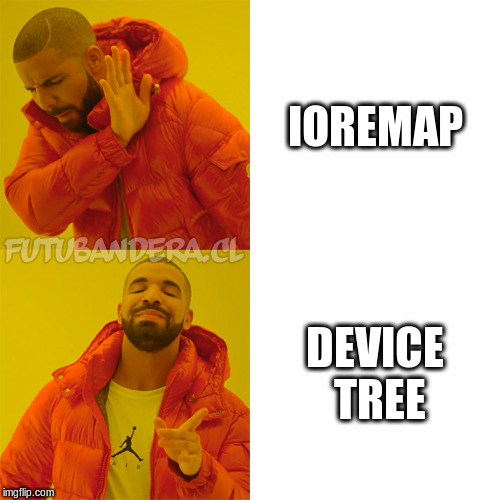
\includegraphics[scale=0.4]{images/ioremap-device-tree.jpg}
  \end{figure}
  \vspace*{-10mm}
\end{frame}

\subsection{Second Attempt}

\begin{frame}[standout]
  \textbf{Attempt \#2} \\
  \vspace{5mm}
  Legacy GPIO API + pinctrl in device tree \\
  \vspace{5mm}
  \alert{DO NOT USE IN REAL LIFE!}
\end{frame}

\begin{frame}
  \frametitle{GPIO Kernel Frameworks}
  \begin{itemize}
    \item Your kernel already has GPIO driver for SoC's GPIO module
      \begin{itemize}
        \item It's platform-dependent: aware of platform-specific data
              (registers, interrupts, etc)
        \item You can't use the driver directly (it's only setting callbacks)
        \item Device Tree definition: \texttt{arch/arm/boot/dts/am33xx.dtsi}
        \item Driver's code: \texttt{drivers/gpio/gpio-omap.c}
      \end{itemize}
    \pause
    \item Kernel has GPIO frameworks to access GPIO driver functions
      \begin{itemize}
        \item Platform-independent API: the same usage for all possible boards
        \item All API calls lead to GPIO driver calls
        \item Legacy GPIO API: \texttt{include/linux/gpio.h}
        \item New GPIO API: \texttt{linux/gpio/consumer.h}
      \end{itemize}
  \end{itemize}
\end{frame}

\begin{frame}[containsverbatim]
  \frametitle{API: Legacy GPIO Kernel API}
  \begin{lstlisting}[language=c,numbers=none]
#include <linux/gpio.h>

int gpio_request(unsigned gpio, const char *label);
void gpio_free(unsigned gpio);
int gpio_to_irq(unsigned gpio);
int gpio_direction_output(unsigned gpio, int value);
int gpio_direction_input(unsigned gpio);
void gpio_set_value(unsigned gpio, int value);
int gpio_get_value(unsigned gpio);
  \end{lstlisting}

  Read \texttt{Documentation/driver-api/gpio/legacy.rst} for details.
\end{frame}

\begin{frame}[containsverbatim]
  \frametitle{Second Attempt: Device Tree}
  \lstinputlisting[caption=am335x-boneblack.dts]{materials/module2/dts.txt}
\end{frame}

\begin{frame}[containsverbatim,allowframebreaks=1]
  \frametitle{Second Attempt: Code}
  \lstinputlisting[caption=hw2.c]{materials/module2/hw2.c}
\end{frame}

\begin{frame}
  \frametitle{Shortcomings}
  Somewhat better, but still has its pitfalls:
  \begin{itemize}
    \item GPIO lines are still hard-coded in driver
    \item Obsolete legacy GPIO API
    \item Referencing pinctrl from \texttt{soc} node is hacky
    \item Still no user space interface
  \end{itemize}
\end{frame}

\section{Assignments}

\begin{frame}
  \frametitle{Assignment 1 (mandatory)}
  \underline{Try out everything we discussed today}:
  \begin{itemize}
    \item Assemble ``LED + button'' device on the breadboard
    \item Build and run provided module \#1 (make sure the device works)
    \item Build and run provided module \#2 (make sure the device works)
    \begin{itemize}
      \item Apply provided patch for \texttt{.dts} file (in kernel)
      \item Rebuild \texttt{.dtb} file for BBB
      \item Boot kernel with new \texttt{dtb} and load \texttt{hw2.ko}
    \end{itemize}
    \item Think about how mentioned problems can be solved
  \end{itemize}
\end{frame}

\begin{frame}
  \frametitle{Assignment 2}
  \underline{Find out and use existing drivers in the kernel}:
  \begin{itemize}
    \item Look for \texttt{gpio-leds} and \texttt{gpio-keys} drivers in
          \texttt{Documentation/devicetree/bindings/}
    \item Try to use those drivers instead of \texttt{hw1.ko} / \texttt{hw2.ko}
          from this lecture
    \item Manage to handle button and LED in user space
    \item How to use PWM module to control LED brightness?
    \begin{itemize}
      \item Which pin to connect LED to?
      \item How to mux that pin for PWM mode?
      \item How to enable PWM module in device tree?
      \item Now how to control the LED brightness from user space? (sysfs)
      \item Which existing driver can be used to control the LED brigtness via
            PWM from device tree? Try to use it.
    \end{itemize}
  \end{itemize}
\end{frame}

\begin{frame}
  \frametitle{Assignment 3}
  \underline{Figure out how \texttt{ioremap()} actually works}:
  \begin{itemize}
    \item Examine \texttt{Documentation/arm/memory.rst}:
    \begin{itemize}
      \item At which addresses \texttt{ioremap()} mappings are stored?
      \item Which function is used to prepare \textit{static mappings}?
    \end{itemize}
    \item Figure out how static mappings are being set up (hint: look where
          the function mentioned in Documentation is being called from
          (from \texttt{arch/} code)? what's passed to that function from
          there?)
    \item Which physical addresses are being statically mapped?
    \item What are the corresponding virtual addresses (calculate manually)?
    \item Look at AM335x TRM, section 2 ``Memory Map'': which hardware modules
          can be accessed via those statically mapped addresses in kernel?
  \end{itemize}
\end{frame}

\begin{frame}
  \frametitle{Assignment 3 (cont'd)}
  \begin{itemize}
    \item Where is that function (from \texttt{arch/}) used? It's set to some
          callback field in some struct. Provide the file path (it's actually
          a \textit{board file}).
    \item What does ``static mapping'' mean? Use \texttt{git blame} on the
          function mentioned in Documentation and read commit messages for found
          commits to get more info. Also Google for it.
    \item Does \texttt{ioremap()} actually creates new MMU mapping in page table
          when you call it, passing some GPIO register address?
    \item Can we avoid using \texttt{ioremap()} in \texttt{hw1.ko}? Why is that
          possible?
    \item Why it's incorrect to use \texttt{ioremap()} for system memory
          (regular RAM)?
  \item Trace \texttt{ioremap()} function call as deep as possible, using your
        IDE capabilities (for BBB architecture)
  \end{itemize}
\end{frame}

\begin{frame}
  \frametitle{Assignment 4}
  \underline{Implement user space GPIO driver for our device}
  \begin{itemize}
    \item Create minimal user space driver (in C) using
          \texttt{/dev/gpiochip*} char devs
      \begin{itemize}
        \item Toggle the LED on button press while your app is running
      \end{itemize}
    \item Look here for insights:
      \begin{itemize}
        \item Syscall interface: \texttt{Documentation/ABI/testing/gpio-cdev}
        \item Examples: \texttt{tools/gpio/*}
      \end{itemize}
    \item It's even better to use \texttt{libgpiod} (you'll have to
          cross-compile it for ARM)
    \item Don't use GPIO sysfs interface, it's obsolete
    \item Send me all source files
    \item \textbf{NOTE}: User-space GPIO interface is useful for makers, but
          usually it's a poor substitute for real kernel drivers
  \end{itemize}
\end{frame}

\begin{frame}[standout]
  Thank you!
\end{frame}

\end{document}
